%% ---------------------------------------------- Chapter Introduction

People need to connect other people, and the urge for connection brings to us what today are known as \glspl{osn}.
These web sites allow us to define a profile as an individual, and to share and visualize content with other individuals in the network, therefore connecting.

\begin{quote}
\textit{"We define Online Social Networks as web-based services that allow individuals to construct a public or semi-public
 profile within a bounded system, articulate a list of other users with whom they share a connection, and view and traverse
 their list of connections and those made by others within the system. The nature and nomenclature of these connections
 may vary from site to site.} \cite{ellison2007social}
\end{quote}

\indent \glspl{osn} have been around for more than a decade now, but these systems have gain world wide popularity since the global adoption of
platforms such as Facebook, Youtube or Twitter, which are platforms that are today massively used across all cultures and age groups, and represents
a paradigm shift on social interaction that we not yet fully understand.\\
\indent The earlier referenced \glspl{osn}, belong to the top of the most visited web sites in the world, that's because these systems not only represents a new
way to keep in touch with friends, but also represents for many, a new way of living, basically we live in network.\\
\indent In this chapter we are going to explore \glspl{osn}, their history, how are these systems being adopted among Internet users, and for some \glspl{osn},
a more detailed and deep study will be conducted for they are important objects of study of this master's thesis.\\
\indent But first, with intent of obtaining a macroscopic perspective of the different \glspl{osn} in the Internet, what they offer
that makes them different from one to another causing many of the users using multiple \glspl{osn} at the same time, we present next a table featuring some
of the most used \glspl{osn}.

%% -------------------------------------------------------------------------------------------- TABLE
\begin{table}[H]
\hspace*{-1.25in}
\renewcommand{\tabcolsep}{2pt}
\begin{tabular}{ |c|c|c|c|l|  }
\hline
\textbf{Name} & \textbf{Year of launch} & \textbf{Registered Users} & \textbf{Active Users} & \textbf{Description/Purpose}\\
\hline
\cellcolor{gray!60}Facebook & 2004 & \textgreater 1 712 000 000 & 1 712 000 000 & \textbf{General}. Photos, videos, blogs, apps.\\
\hline
\cellcolor{gray!60}Google+ & 2011 & 1 600 000 000 & 300 000 000 & \begin{tabular}{@{}l@{}}\textbf{General}. Google+ is an interest-based\\social network that is owned\\and operated by Google.\end{tabular}\\
\hline
\cellcolor{gray!60}Youtube & 2005 & \textgreater 1 000 000 000 & 1 000 000 000 & \begin{tabular}{@{}l@{}}Allows billions of people to discover,\\watch and share originally-created videos.\\Provides a forum for people to connect,\\ inform, and inspire others.\end{tabular}\\
\hline
\cellcolor{gray!30}Qzone & 2005 & \textgreater 652 000 000 & 652 000 000 & \begin{tabular}{@{}l@{}}\textbf{General}. It allows users to write blogs,\\keep diaries, send photos, listen to music,\\and watch videos.\\It's only available in Chinese.\end{tabular}\\
\hline
\cellcolor{gray!30}Twitter & 2006 & 645 750 000 & 313 000 000 & \textbf{General}. Micro-blogging, RSS, updates.\\
\hline
\cellcolor{gray!30}Tumblr & 2007 & \textgreater 555 000 000 & 555 000 000 & \begin{tabular}{@{}l@{}}Microblogging platform and social networking website.\end{tabular}\\
\hline
\cellcolor{gray!30}Instagram & 2010 & \textgreater 500 000 000 & 500 000 000 & A photo and video sharing site.\\
\hline
\cellcolor{gray!30}LinkedIn & 2003 & \textgreater 450 000 000 & 106 000 000 & Business and professional networking.\\
\hline
\cellcolor{gray!30}Sina Weibo & 2009 & 300 000 000 & 282 000 000 & \begin{tabular}{@{}l@{}}Social microblogging site in mainland China.\end{tabular}\\
\hline
\cellcolor{gray!30}VK & 2006 & 249 409 900 & 100 000 000 & \begin{tabular}{@{}l@{}}\textbf{General}, including music upload, listening and search.\\Popular in Russia and former Soviet republics.\end{tabular} \\
\hline
\cellcolor{gray!30}Reddit & 2005 & 234 000 000 & 120 000 000 & \begin{tabular}{@{}l@{}}Social media, social news aggregation, web\\content rating, and discussion website.\end{tabular}\\
\hline
\cellcolor{gray!30}Vine & \textbf{2013} & 200 000 000 & 100 000 000 & \begin{tabular}{@{}l@{}}Short-form video sharing service where\\ users can share six-second-long looping video clips.\end{tabular}\\
\hline
\cellcolor{gray!30}Pinterest & 2010 & 176 000 000 & 100 000 000 & \begin{tabular}{@{}l@{}}The world’s catalog of ideas. Find and save\\recipes, parenting hacks, style inspiration and\\other ideas to try.\end{tabular}\\
\hline
\cellcolor{gray!30}Flickr & 2007 & 112 000 000 & 92 000 000 & \begin{tabular}{@{}l@{}}Helping people make their photos\\ available to the people who matter to them.\\Enable new ways of organizing\\photos and video.\end{tabular}\\
\hline
\cellcolor{gray!10}Meetup & \textbf{2002} & 27 590 000 & - & \begin{tabular}{@{}l@{}}World's largest network of local groups.\\Meetup makes it easy for anyone\\to organize a local group or find\\one of the thousands already meeting\\up face-to-face. \cite{meetup}\end{tabular}\\
\hline
\cellcolor{gray!10}Couchsurfing & 2004 & 12 000 000 & - & \begin{tabular}{@{}l@{}}Couchsurfing connects travelers with\\a global network of people willing\\to share in profound and meaningful ways,\\ making travel a truly\\ social experience. Is commonly used by travelers\\to find free hosts across the globe.\\\cite{csurf}\end{tabular}\\
\hline
\cellcolor{gray!10}ResearchGate & 2008 & \textgreater 11 000 000 & - & \begin{tabular}{@{}l@{}}Built by scientists, for scientists.\\Connect the world of\\ science and make\\ research open to all. \cite{rgate}\end{tabular}\\
\hline
\end{tabular}
\caption{\label{table:osns} Table describing most used \glspl{osn}. (\cite{statista}, \cite{expandedramblings})}
\end{table}
%% -------------------------------------------------------------------------------------------- TABLE

\indent Table \ref{table:osns} lists the most used and popular \glspl{osn}, \textbf{ordered by the estimated number of registered users}.
Also notice that, for those \gls{osn} where the number of registered users is unknown, we will assume that it is a larger value than
the monthly active users represented by the column \textit{Active Users}.
\\
\indent The first obvious comment on the listed \glspl{osn} is that general purpose \glspl{osn} have more users (social
networks with the word \textit{General} in bold), being Youtube an exception, since it is not a general purpose \glspl{osn}, neither
is focused on individuals, it is build around \textbf{social objects}, the videos.
\\
\indent The grey scale in the first column of Table \ref{table:osns} divides \glspl{osn} in three groups: the first and smallest, the 1 billion
or more users \glspl{osn}; the second the \glspl{osn} with less than 1 billion users and more then 100 million; finally, the third group, \glspl{osn} with
less then 100 million users. At this point, we begin to observe that \textbf{the narrower purpose \glspl{osn}} such as ResearchGate (mainly for researchers) or
Couchsurfing (mainly for open minded travelers), \textbf{have a smaller number of registered users}, which is expected since the target audience is also smaller.
\\
\indent Other \glspl{osn} not listed in Table \ref{table:osns}, but still worth mentioning include \textbf{Classmates} (helps users finding
classmates form kindergarten, primary school, high school etc.) known for being one of the first \glspl{osn}, since it was
launched in 1995, and \textbf{Ask.fm} (allows users to interact with other users asking and answering questions (revealing identity is optional)).
\\
\indent An important note on the listed \glspl{osn} in Table \ref{table:osns} is that only Qzone, Vine, Couchsurfing and ResearchGate don't provide any web APIs
to fetch data or publish content, while all the others offer a wide variety of web services for developers to consume and use as they please, of course within the terms and policies
of use of each \gls{osn}.

%% ---------------------------------------------- History of Online Social Networks
\section{History of Online Social Networks}
\begin{figure}[h!]
\begin{center}
  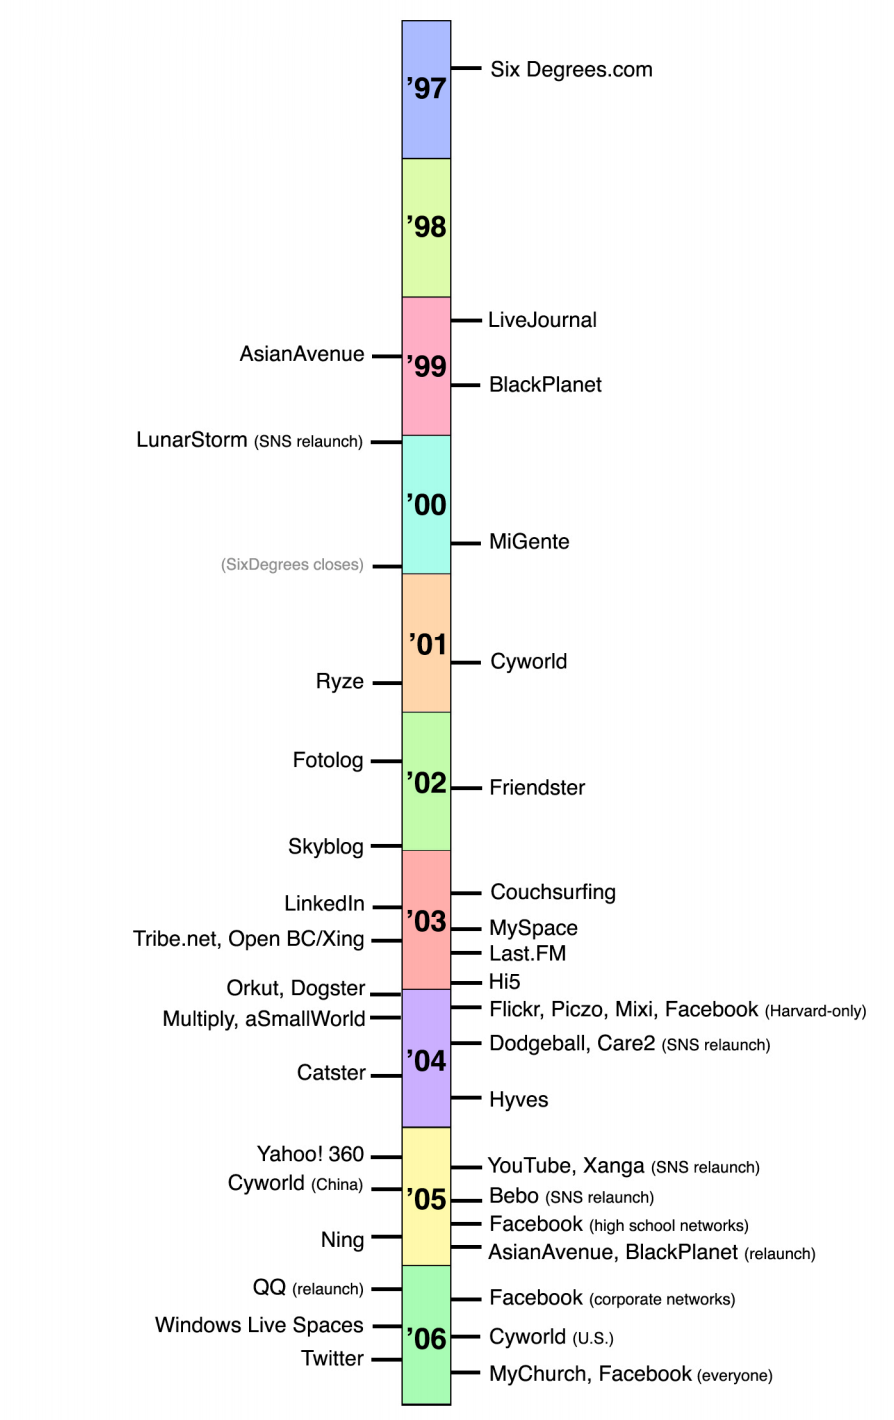
\includegraphics[width=0.7\textwidth]{img/timeline.png}
\end{center}
\caption{\label{img:timeline} Launch dates of major \glspl{osn}. (\cite{ellison2007social})}
\end{figure}

Although the first platform possessing some of the main characteristics that define \glspl{osn},
according to \cite{ellison2007social}, the first recognizable \gls{osn} launched in 1997 as we can observe in the Figure \ref{img:timeline}. \textit{SixDegrees.com} allowed users to create personal
profiles, connect with friends and consult friends of friends lists. The profile feature came from the
online dating sites and online communities, while the surfing trough register users in the network
and consulting friends was an existing feature in Classmates.com. \textit{SixDegrees.com} was the first to combine
these features.

\textit{SixDegrees} promoted itself as a tool to help people to connect, but in 2000, it became an
unsustainable business and the service closed. At the time the creators conclude that
\textit{SixDegrees} was a service that was very ahead of its time.

Until 2002 many \glspl{osn} have emerged, but still incapable of projecting themselves at a global scale.
As we can observe in the timeline of Figure \ref{img:timeline} from 2002 and 2005 the \textit{big players} came to existence, in these period, \gls{osn}
such as Friendster, LinkedIn, MySpace, Hi5, Facebook and Youtube were born, shaping the business, cultural
and research landscape.


%% ---------------------------------------------- Portuguese and Online Social Networks
\section{Portuguese People and Online Social Networks}
From Table \ref{table:osns}, we get a good overview on \glspl{osn} usage among modern society. In this section we do a deep exploration of the most adopted \glspl{osn} by portuguese citizens,
and get to compare then with the more global scenario presented in Table \ref{table:osns}, also, other interesting facts will be revealed where appropriate.\\
\indent A recent study, \cite{marktest2016}, revels portuguese relationship with \glspl{osn}. This study, has been made by \textit{Marktest Consulting} since 2011, with the goal of know the notoriety, utilization, opinion
and habits of portuguese concerning social networks. The study information was collected trough online interviews. The sample was built from 819 interviews from individuals with age between
15 and 64 years, living in Portugal and using \glspl{osn} in a daily basis.\\
\indent Some of the most interesting facts revealed in this study, relative to the participants are:
\begin{itemize}
  \item 94\% has a Facebook account and 43\% a Youtube account;
  \item 21\% has abandoned a social network in the past year;
  \item 27\% considers that their dedicated time to social media has increased;
  \item 67\% follows celebrities and 62\% follows brands;
  \item 87\% is used to watch videos in social networks.
\end{itemize}

\indent These are indeed interesting conclusions, but what about the top used \glspl{osn}, \textbf{the most used are
the following (by order): Facebook, Youtube, Google+, LinkedIn, Instagram and Twitter}.\\
\indent Relatively to \cite{marktest2016} past studies, Facebook has maintain
its top position, maintaining a grow tendency that has been standing out in the past years.

\indent Going back to Table \ref{table:osns}, we may now comment the usage of \glspl{osn} by portuguese people comparing it
to the global scenario. As one may notice Facebook still rules users preferences within portuguese.
The other noticeable point is that the \glspl{osn} preferred among portuguese are general propose ones,
but with a slight tendency to content sharing networks (mainly photos).

\indent Concerning to global time related usage statistics, according to \cite{marktest2016}, \textbf{portuguese spend 91 minutes a day with social networks},
68\% considers that this is the ideal time to spent with social media, despite 1 in each 4 saying that in the past year has dedicated even more time to them.
Even if people spent more than one hour and an half in this platforms, the study
concluded that \textbf{67\% of the users that visit \glspl{osn} several times a day only 41\% does daily publications}.

\indent \textbf{The prime time for using \glspl{osn} is between 8pm and 10pm}, being the smartphone the most used device in this time. Also in this short period the
featured \gls{osn} is Facebook, the majority of the interviewed say that is the most credible site, the one that provides better and useful information,
the most interesting and addictive.


%% ---------------------------------------------- Exploring Some OSNs
\section{Exploring Specific Online Social Networks}

In this section we are going to explore in greater detail some of the \glspl{osn} presented
in Table \ref{table:osns}. The selection of the social networks was not aleatory, we are going
to study deeply the \glspl{osn} that gather some important characteristics, that will be of use in
the future when we design the system for analyzing and visualizing social networks. First, the
\gls{osn} must be accessible, this said, one must be capable of extracting information from the platform
in order to analyze it. Second, the \glspl{osn} must be the most diversified as possible, so that we
can draw different types of conclusions derived from different kind of analysis, for then give proof
of the adaptability of the system to different \glspl{osn}. Considering the previous
comments, these are the following \glspl{osn} that will study with more detail:
\begin{itemize}
  \item Facebook
  \item Instagram
  \item LinkedIn
  \item ResearchGate
  \item Pinterest
\end{itemize}

%% ---------------------------------------------- Exploring Some OSNs
%% -------------------------------------------------- Facebook
\subsection{Facebook}

Facebook is an \gls{osn}, created by Mark Zuckerberg in 2004, which started out by being an exclusive social network for Harvard students, but came later to spread across
the country and the globe, having today more than one billion users.\\
\indent Before diving into details of Facebook's domain, one must first point out some of its general aspects. Facebook basically allows anyone with a valid email address to create a public and personalized profile,
we say personalized in terms of displayed content or information such as profile photo, name, work, homeland, education etc. .
The next fundamental step is connect with other users, by sending friendship requests to other Facebook users (this are bidirectional relations).
The base entity of the network is the user, but entities such as brands, companies can also be part of the platform, appearing normally
in the form of page, being a page a public place inside the network with marketing or business related purposes (celebrities, public institutions also use pages as form of appearing in Facebook).\\
\indent The next parts of this section will clarify the roles of this entities and their way of interact with each other, also other important concepts will be presented.

\subsubsection*{Domain Model}

\begin{figure}[h!]
  \hspace*{-1in}
  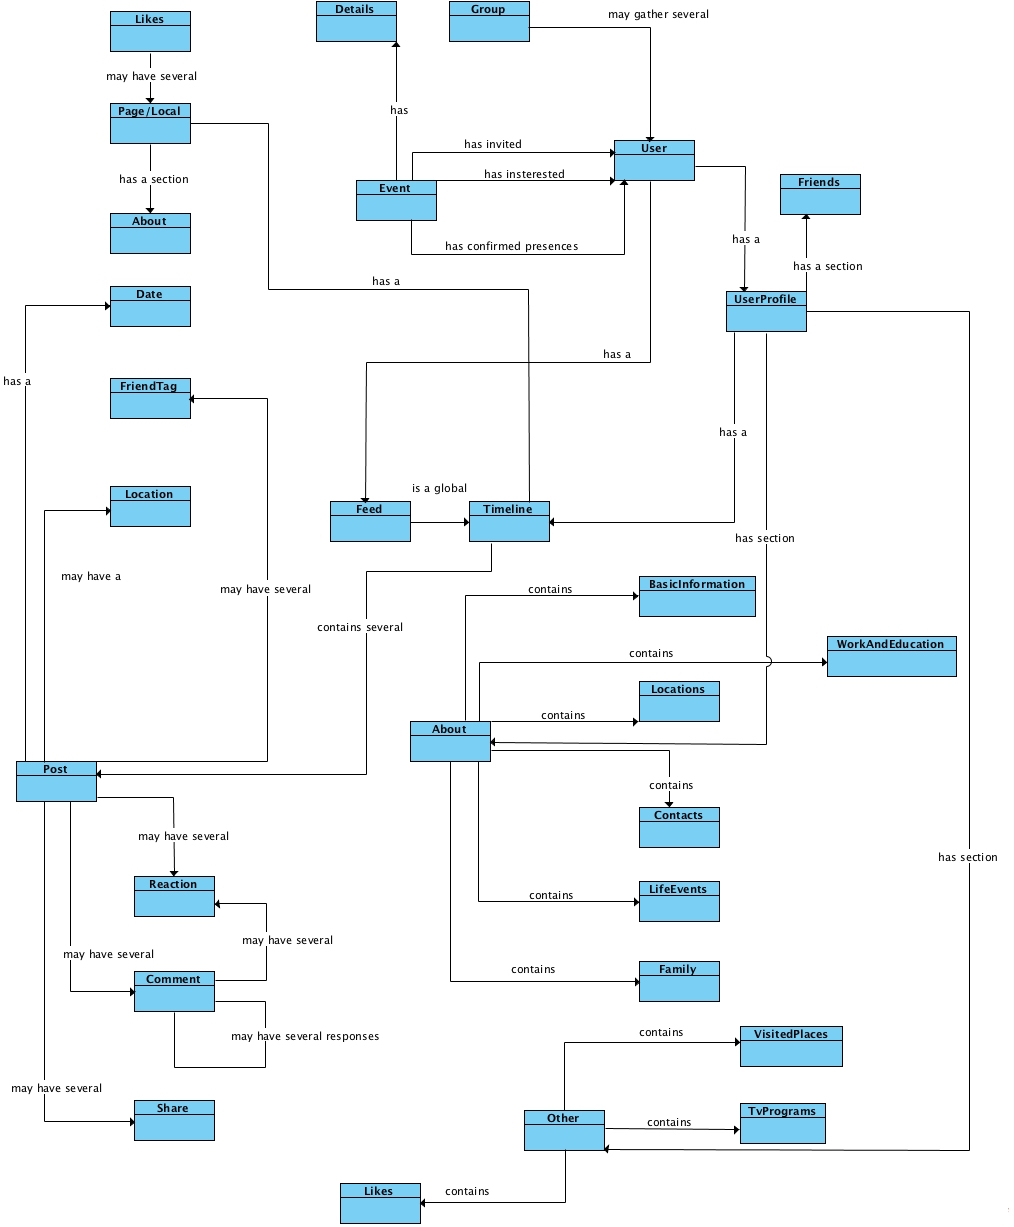
\includegraphics[width=1.28\textwidth]{img/facebook-domain-model.jpg}
\caption{\label{img:fbdomain} Facebook domain model schema.}
\end{figure}

\indent In this section we explore the domain of Facebook represented in Figure \ref{img:fbdomain} in detail, what are the pieces that conceptually build
this platform, and how they relate. The schema in Figure \ref{img:fbdomain} represents a macroscopic perspective among Facebook components and their organization.\\
\indent There are two entities with bold labels in the schema, this are, \textbf{User} and \textbf{Post}, being
\textit{User} the base entity in the network (the node in the network graph basically), and \textit{Post} the most basic unit of content sharing in Facebook.\\
\indent Facebook is interesting in terms of data gathering, because despite offering users' basic information
and to whom that users are related (\textit{Friends} box), it has a collection of other interesting data
such as the family relationships (\textit{Family} box), geographical locations where the user lives, or
visited locations (\textit{Locations} and \textit{VisitedPlaces} boxes respectively), and among other things, user information
may contain the personal interests that were explicitly inputed by the user (\textit{Likes} box).\\
\indent In what concerns to user activity in the platform, the \textit{Timeline}, provides all the user
Posts chronologically ordered, this is where Facebook dynamism takes place, users are constantly
adding content to their timeline, it may be life related events or simply sharing other users posts linking content.\\
\indent Facebook has, with time, become more then a user profile centralized network, it has invested in expand its horizons, becoming
the place where pages of brands, companies, organizations (media, political, non-profitable etc.), or places (cities, monuments, bars etc.) live (\textit{Page/Local} box).
This entities that are now cohabiting with users in the Facebook ecosystem, take advantage of the platform and its range to get their updates to most people as possible. The profile
for these pages are in many ways different form the user's profile, it also has a timeline, but the about information and other details represent a smaller part of page's profiles,
the most important metric for pages is its number of \textit{likes} (\textit{Likes} box), it represents the number of users in the network that follow the page, it might be users
that simply have a certain relation with the entity or simply want to keep in touch by regularly receiving these entities updates in their Facebook walls
\footnote{Facebook wall an area where users can see the posts of their friends and/or liked pages, in a chronological order}.\\
\indent Other Facebook entities not yet mentioned, are events (\textit{Event} box). These are events inputed in the platform that allow
users to keep updated about relevant events happening mainly in their area. Users can tag the event as \textit{interested in}, showing their friends
the will of participating in some event, or they can simply reject the event. Users also can confirm participation on events
showing their network that they will be present. Events keep three separated counters for users, they count the number of invited users, number of
interested users and number of confirmed users (these relations are expressed as links between the \textit{Event} box and the \textit{User} box).\\
\indent In Facebook is also possible to join groups of users, this groups may be public or private, and they generally are focused on a specific matter,
or gather users from one same institution or organization (e.g. Facebook group of students of the University of Minho).
Having this feature of groups, clustering users by they interests one may say that groups, some way, transform Facebook in a "multi interest-based \gls{osn}".

\subsubsection*{Facebook Graph API}
Facebook has today several software \textit{kits} for developers to interact with the platform in the most diversified and imaginable ways. Facebook developers
offers a range of variated software products that vary from monetization programs, that focus on how to make users profit from Facebook, Analytics to developers who
have their apps embedded in the Facebook platform understand their audience and the performance of their apps, etc. (\cite{fbproducts}).\\
\indent In this master's thesis context, the relevant software that Facebook has available is the Facebook Graph API. This API basically allows developers to collect information
from Facebook such as posts, photos, videos, pages etc. According to \cite{fbgapi}, the common scenarios for using the Graph API
are the following: determine whether two people are friends on Facebook; publishing new status and updates, uploading content (photos, video etc.); sharing links. But in this project what we seek is
build the most biggest and detailed network as possible, with analysis and visualization purposes in mind.\\
\indent For building the network fetching users friends information is crucial, this was possible until Facebook Graph API v2.0 (trough the router \textit{/me/friends}), one could actually retrieve
friends information and build a network from there. From v2.0 on, to achieve what was explained before, one must request a special permission called \textbf{user\_friends}
from each user. The permission \textbf{user\_friends} is no longer included by default in every login. This change breaks down the possibility of gather Facebook information via its Graph API,
this said, we need in the future to look up alternative paths to extract data from Facebook.


%% ---------------------------------------------- Exploring Some OSNs
%% -------------------------------------------------- Instagram
\subsection{Instagram}

\begin{quote}
\textit{"Since the beginning, Kevin has focused on simplicity and inspiring creativity through solving problems with thoughtful
product design. As a result, Instagram has become the home for visual storytelling for everyone from celebrities, newsrooms and
brands, to teens, musicians and anyone with a creative passion."} \cite{instabout}
\end{quote}

Similarly to Facebook we are going to explore Instagram in the same way. Instagram was originally developed by Kevin Systrom and Mike Krieger, and launched in 2010, only
for iPhone devices. Within a year Instagram was able to gather around 10 million of users. Later, in 2012 Facebook acquire Instagram for approximately 1 billion dollars.\\
\indent As already mentioned in Table \ref{table:osns}, does not belong to the group of general purpose \glspl{osn}, instead, Instagram specially focused on photo
and video sharing, building a global community that shares more than 95 million photos every day.\\
\indent According to \cite{instabout}, since
the very beginning Instagram was a very simplistic platform, being this characteristic reflected on its domain model.

\subsubsection*{Domain Model}

\begin{figure}[h!]
  \hspace*{-1in}
  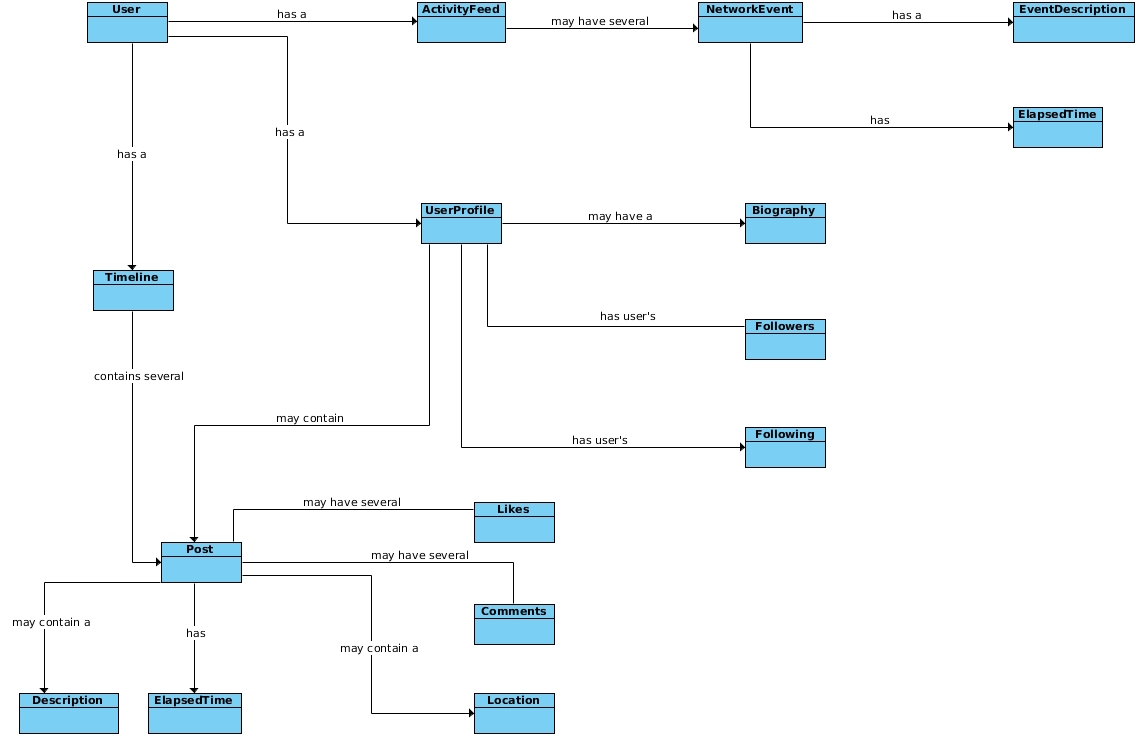
\includegraphics[width=1.28\textwidth]{img/instagram-domain-model.jpg}
\caption{\label{img:instadomain} Instagram domain model schema.}
\end{figure}

Figure \ref{img:instadomain} represents the domain model of Instagram, and as we can observe, simplicity its the essence of this platform, since this diagram is far
more a realistic representation of Instagram than Figure \ref{img:fbdomain} is a representation of Facebook, and this may be why Instagram is so massively adopted by users
on the Internet, because it goes directly to the point, focusing mainly on sharing activity, offering a real easy and simple user experience.\\
\indent Now concerning to the domain model, we can see that a user and its profile (\textit{User} and \textit{UserProfile} boxes) are very simple entities, because
a user's profile is only its biography (\textit{Biography} box), relationships (\textit{Followers} and \textit{Following} boxes) and the user's posts, that despite
being chronologically ordered, do not intend to form any kind of timeline such as Facebook, instead it represents more the concept of a wall with frames hanged on it.\\
\indent In Instagram the landing page, represents a timeline (\textit{Timeline} box) with posts from users we follow. Regarding to posts (\textit{Post} box), one can
comment posts (\textit{Comment} box), but one cannot react or respond to comments (this preserves simplicity even more, for nested comments represent
 a complex part of \gls{osn} such as Facebook), and react to them by the \textit{like} reaction (\textit{Like} box).

\subsection*{Instagram API Platform}
In consequence of a simple domain, Instagram API Platform, provides simple and useful
end points for programmatic publishing, and for network discovering, as far as concerning to this project, the late utility
is more of interest. Instagram allows to get users, their relationships and also the media shared content (posts).\\
\indent Similarly when exploring Facebook Graph API, we now found also very intimidating restrictions for the purpose of this project,
this restrictions include limited rate of 500 API requests per hour, and end point specific limitations that allow only to
perform 30 requests per hour to getting users' relationships data. (\cite{instadev})

%% ---------------------------------------------- Exploring Some OSNs
%% -------------------------------------------------- LinkedIn
\subsection{LinkedIn}

Moving on to the next \gls{osn} we now have LinkedIn. According to \cite{linkabout}, LinkedIn was launched officially on May 5 of 2003, and by the end of
that month, the network had already more than 4500 members. In 13 June of 2016 LinkedIn was acquired by Microsoft in an all-cash transaction valued at \$26.2
billion (\cite{microlink}).\\
\indent LinkedIn is an \gls{osn} that has a very narrow purpose, which is
connecting professionals around the globe to make them more productive and successful.

\subsubsection*{Domain Model}

\begin{figure}[h!]
  \hspace*{-1in}
  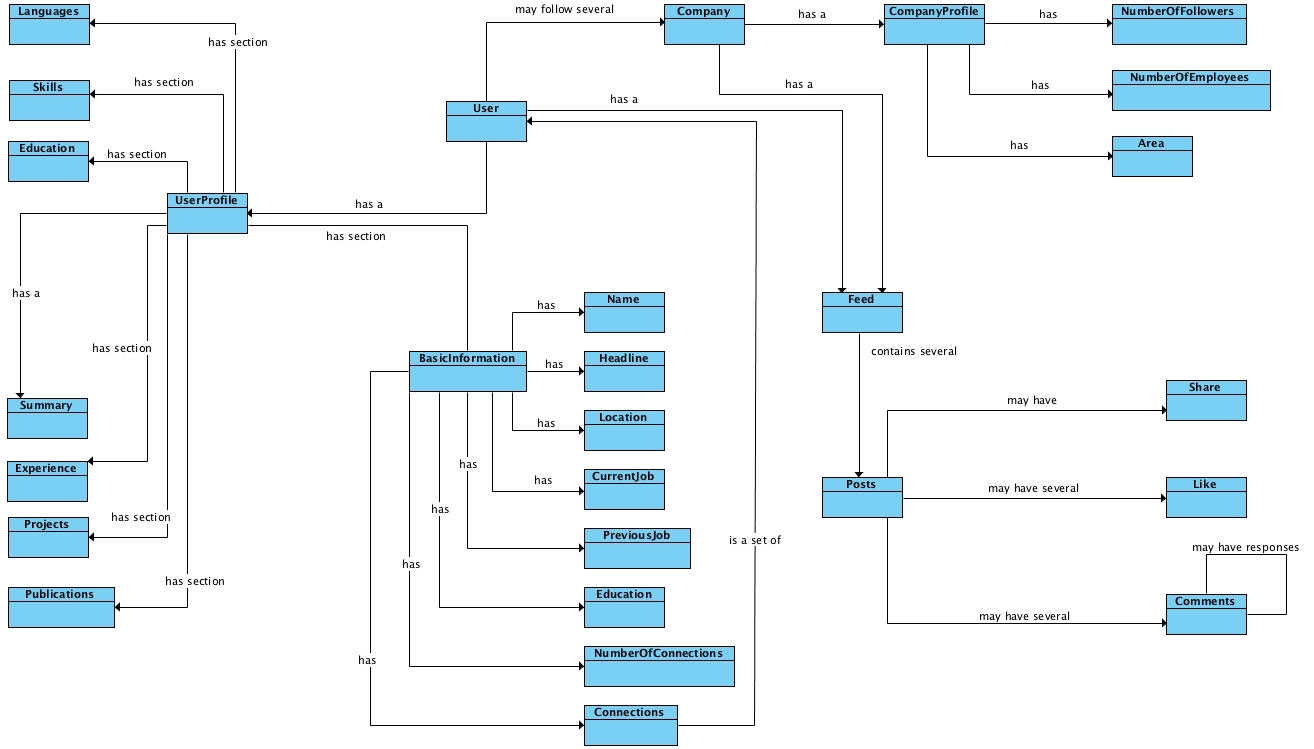
\includegraphics[width=1.20\textwidth]{img/linkedin-domain-model.jpg}
\caption{\label{img:linkdomain} LinkedIn domain model schema.}
\end{figure}

\indent Being a more purpose oriented \gls{osn} and focused on the professional
world, makes LinkedIn platform more complex, even with a simplified representation of the domain model, as we can observe in Figure \ref{img:linkdomain} it is schema
\footnote{\indent In the schema presented on Figure \ref{img:linkdomain}, much of the platform complexity was simplified in order to produce a simple domain, and to narrow
down this analysis to the core components and concepts of LinkedIn.}
far more complex that Instagram, having more or a similar complexity comparing to Facebook.\\
\indent In LinkedIn the user profile (\textbf{UserProfile} box) is very rich in terms of what is important for building an individual professional image (profile),
starting by one individual's basic information (\textbf{BasicInformation} box) that has information like name, location and current and/or previous jobs. Then
the user profile has several sections with very specific purposes such as professional experience (\textbf{Experience} box), languages (\textbf{Languages} box) or
education (\textbf{Education} box), all this summed up give a very precise perspective of an individual's "professional appearence". At the bottom of the profile
we have along with the professional recommendations and connections, the skills or expertise section (\textbf{Skills} box), this is one of the most attractive features
in the LinkedIn platform. Skills in LinkedIn are a tagging system that allow user's to expose their expertise trough their public profile and then receive feedback
on them according to their ability on that specific skill, this is a very important and promising feature for matching user's profiles with
job positions requirements.\\
\indent LinkedIn's main entities are not only users, the industry is massively represented in this network too. Companies may have a company profile
(\textbf{Company} and \textbf{CompanyProfile} boxes) where they present the company, containing basic information such as number of people following the company
number of employees (giving the idea of the company dimension) and the area where the company fits (pharmaceuticals, technology etc.) (\textbf{NumberOfFollowers},
\textbf{NumberOfEmployees} and \textbf{Area} boxes respectively).\\
\indent Other important concept of LinkedIn is the user feed where the user can chronologically consult a series of posts produced by their connections
or by companies that their follow.

\subsection*{LinkedIn API}
LinkedIn provides a REST API (\cite{linkapi}), but still similarly to the \glspl{osn} we been studying its very limited. In what concerns to data retrieval LinkedIn only allows
the consult of basic profile data, this is the data retried from the LinkedIn interactive REST console:\\

\begin{verbatim}
  {
  "firstName": "Daniel",
  "headline": "Graduate Front-end Developer at Blip.pt",
  "id": "k_yk8W37WH",
  "lastName": "Caldas",
  "siteStandardProfileRequest":  {
    "url": "https://www.linkedin.com/profile/..."
  }
\end{verbatim}

%% ---------------------------------------------- Exploring Some OSNs
%% -------------------------------------------------- ResearchGate
\subsection{ResearchGate}

\begin{quote}
\textit{"Founded in 2008 by physicians Dr. Ijad Madisch and Dr. Sören Hofmayer, and computer scientist
Horst Fickenscher, ResearchGate today has more than 11+ million members. We strive to help them make progress happen faster."} \cite{rgate}
\end{quote}

ResearchGate is an \gls{osn} built specifically for scientists, with the goal of easing the task of collaborative research around the globe. ResearchGate
strikes to connect the world of science and make research open to all.

\subsubsection*{Domain Model}

\begin{figure}[h!]
  \hspace*{-1in}
  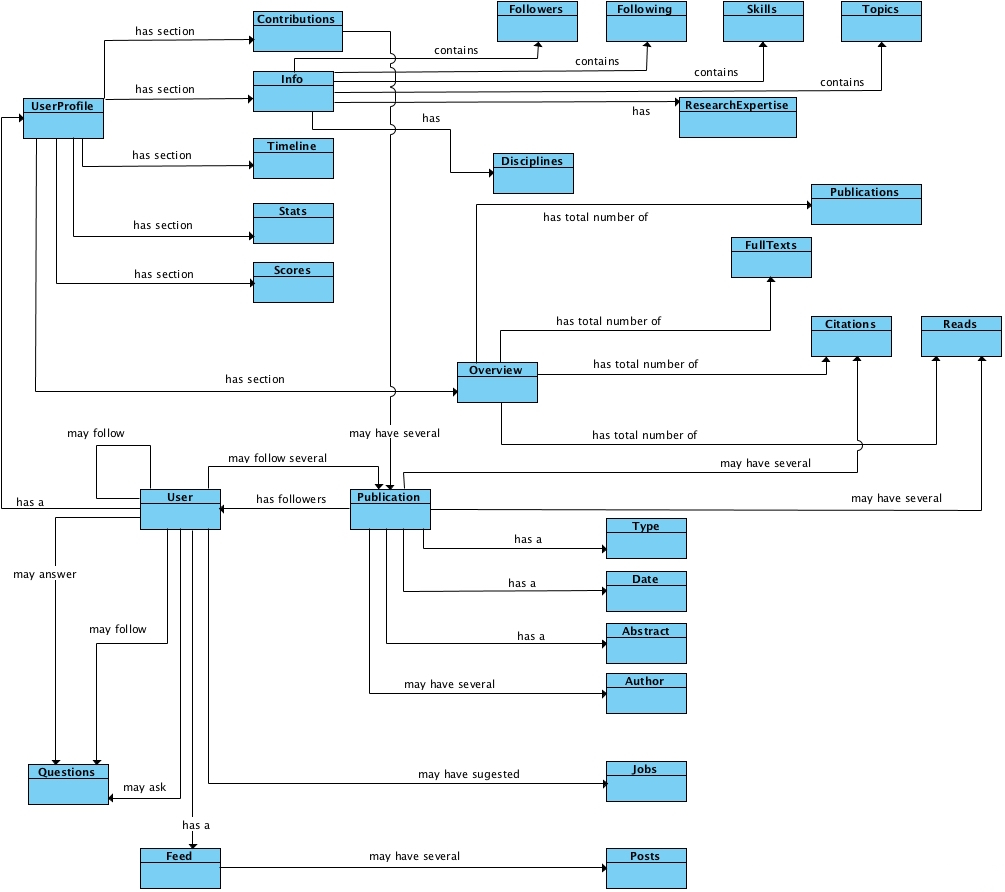
\includegraphics[width=1.20\textwidth]{img/researchgate-domain-model.jpg}
\caption{\label{img:rgatedomain} ResearchGate domain model schema.}
\end{figure}

\subsubsection*{Data Dictionary}
Some terms on the schema presented in Figure \ref{img:rgatedomain} may be quite ambiguous due to the the specificity that they represent. In order to make the schema fully legible and before diving into the domain model analysis, we present first, a small data dictionary detailing the terms one may found more ambiguous:

\begin{itemize}
\item \textbf{Scores} - This term represents a collection of metrics that evaluate the performance of a user based on his contributions and research experience. The user has also associated a global score;
\item \textbf{Topics} - Topics represent the user's scientific areas of interest, ResearchGate uses topics to provide personalized suggestions;
\item \textbf{Disciplins} - Represent more broad areas of the user education,
expertise and interest;
\item \textbf{Type} \begin{small}(\textbf{Type} box connected with the \textbf{Publication} box in Figure \ref{img:rgatedomain})\end{small} - A type classifies a publication, this said, a publication may be an article, a book, a thesis a conference paper etc. .
\end{itemize}

\subsubsection*{Domain Model Analysis}
ResearchGate is a peculiar \gls{osn} that despite having connections between individuals, it has alongside connections between individuals and scientific publications,
making the publication (\textbf{Publication} box) a social object, playing the same role that videos play in Youtube for example.\\
\indent Like LinkedIn the user profile (\textbf{UserProfile} box), is very detailed and builds up a very clear image of the researches work, positions and areas of interest. The relations
among users are bidirectional, following the followers/following (\textbf{Followers} and \textbf{Following} box) strategy like other \glspl{osn} such as Instagram or Twitter. Very simillarlly to LinkedIn, a
user's profile has a skills (\textbf{Skills} box) section, where skills are expressed in the form of tags, the tag description is far more specific than LinkedIn tags, that may some
times acquire very abstract or high level descriptions (e.g. Technology Information). In ResearchGate tags have are very specific and are
normally related with the user topics (\textbf{Topics} box) or disciplines.\\
\indent Publications play along with the user a main role in ResearchGate. Normally publications have associated a type (already explained in the data dictionary section), a date, an abstract and may have one or more authors. The main metrics for Publications rating are the number of reads (\textbf{Reads} box) and the number of
citations (\textbf{Citations} box) of that publication. The publications may also be followed by users that may have interest on particular publications.\\
\indent Other concept of ResearchGate that raises the collaborative spirit among users, living up to the values that originated the platform, is the questioning system
(\textbf{Question} box). Users may ask each other specific questions and have them answered by an expert on a specific scientific area, this opens up the possibility of having
the best experts on a specific matter giving their opinion, thus the possibility of obtaining the "best answer possible in the globe".\\
\indent ResearchGate users' receive open jobs suggestions based on their profile, also user's have a post where they receive activity notifications of the people
or publications that they are following.

\subsubsection*{API}
Today ResearchGate does not provide any API for accessing its data or for any kind of interaction with the platform.

%% ---------------------------------------------- Exploring Some OSNs
%% -------------------------------------------------- Pinterest
%\subsection{Pinterest}
%...

%% ---------------------------------------------- How Social Networks Have Changed The World
%\section{How Social Networks Have Changed The World}
%...
% Cool overview: https://www.youtube.com/watch?v=trH4iuebjjI
% What really changed? What people did that was good that people don't do anymore? A general overview to the impacts of OSNs!
